
\begin{figure}
\centering
\begin{subfigure}{.50\textwidth}
\centering
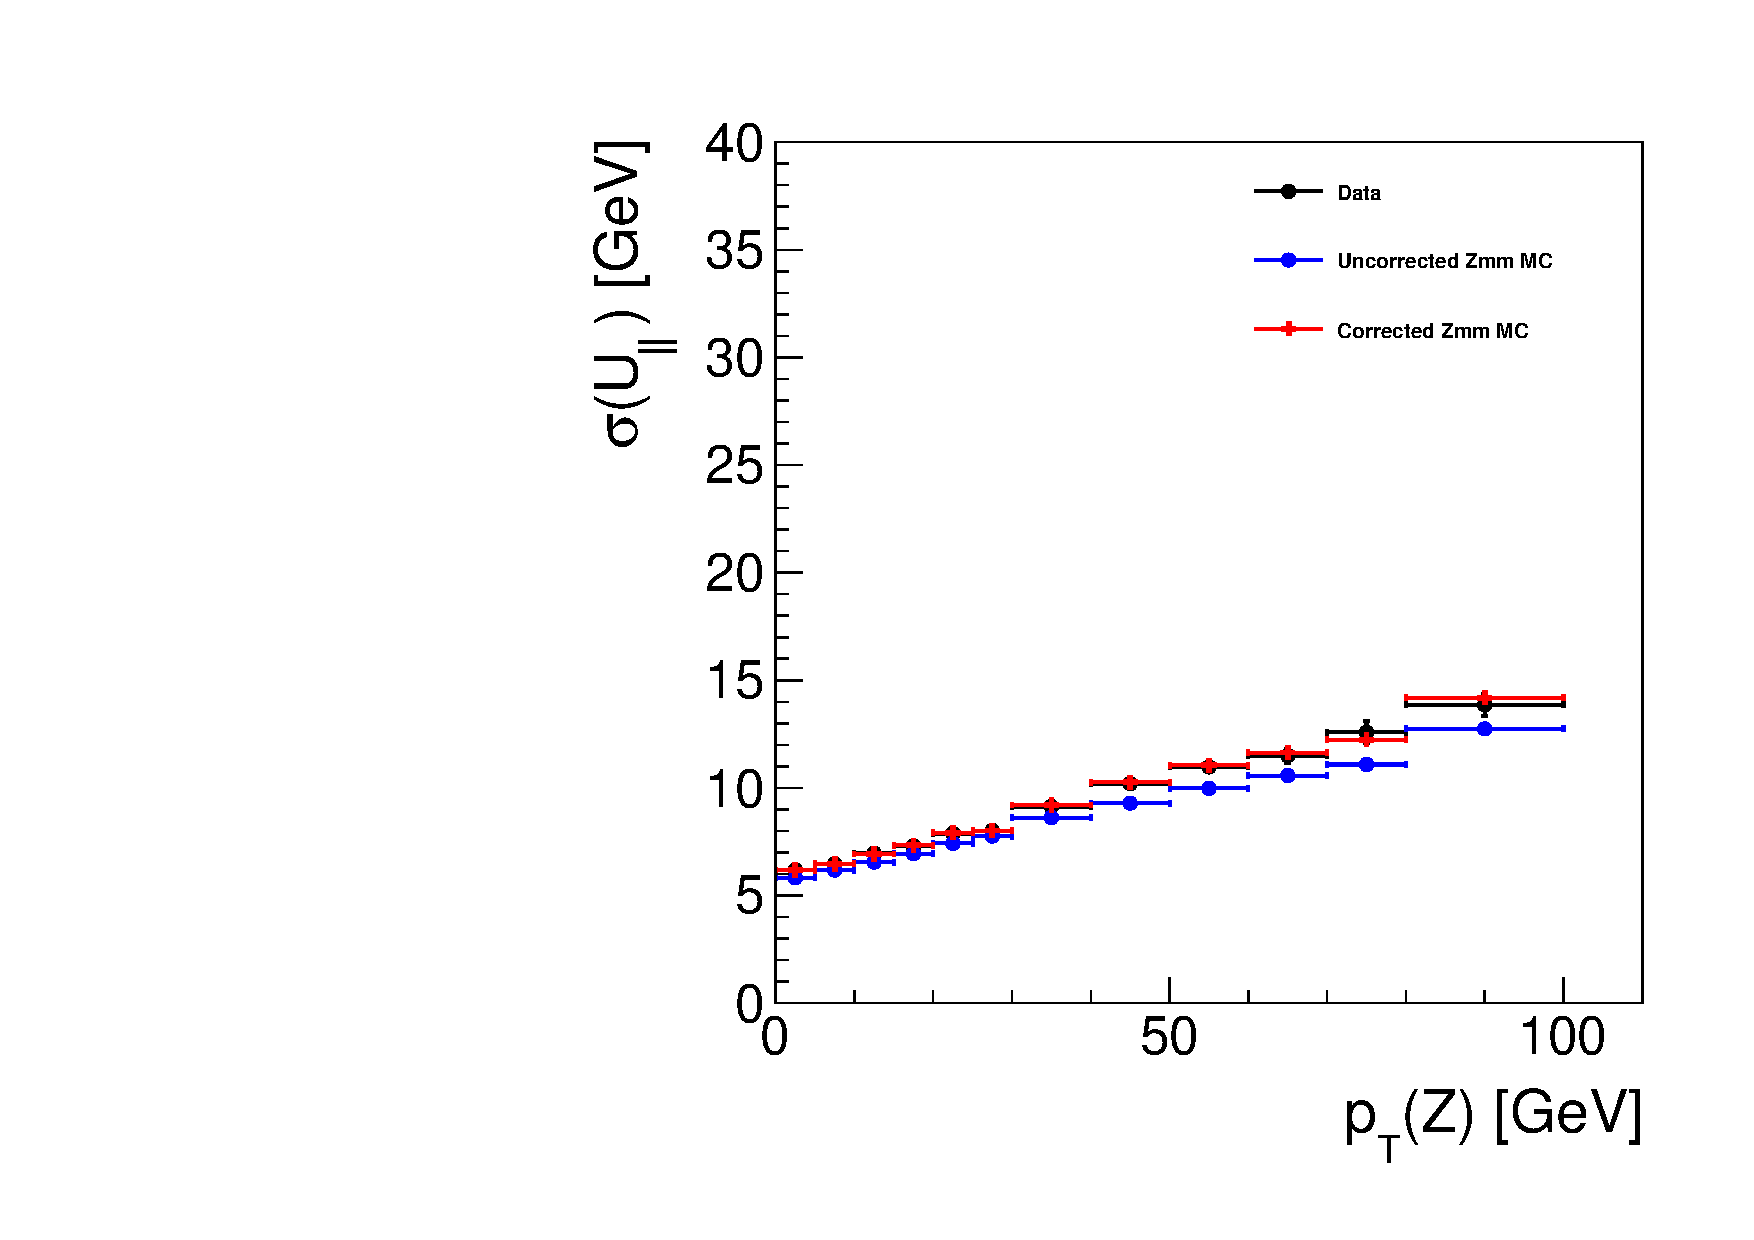
\includegraphics[width=\linewidth]{plots/Recoil/validation_5/resolution_par.pdf}
 \caption{Resolution of \upar}
%   \label{fig:Eff:el:5TeV:GSFSel:pos
\end{subfigure}%
\centering
\begin{subfigure}{.50\textwidth}
\centering
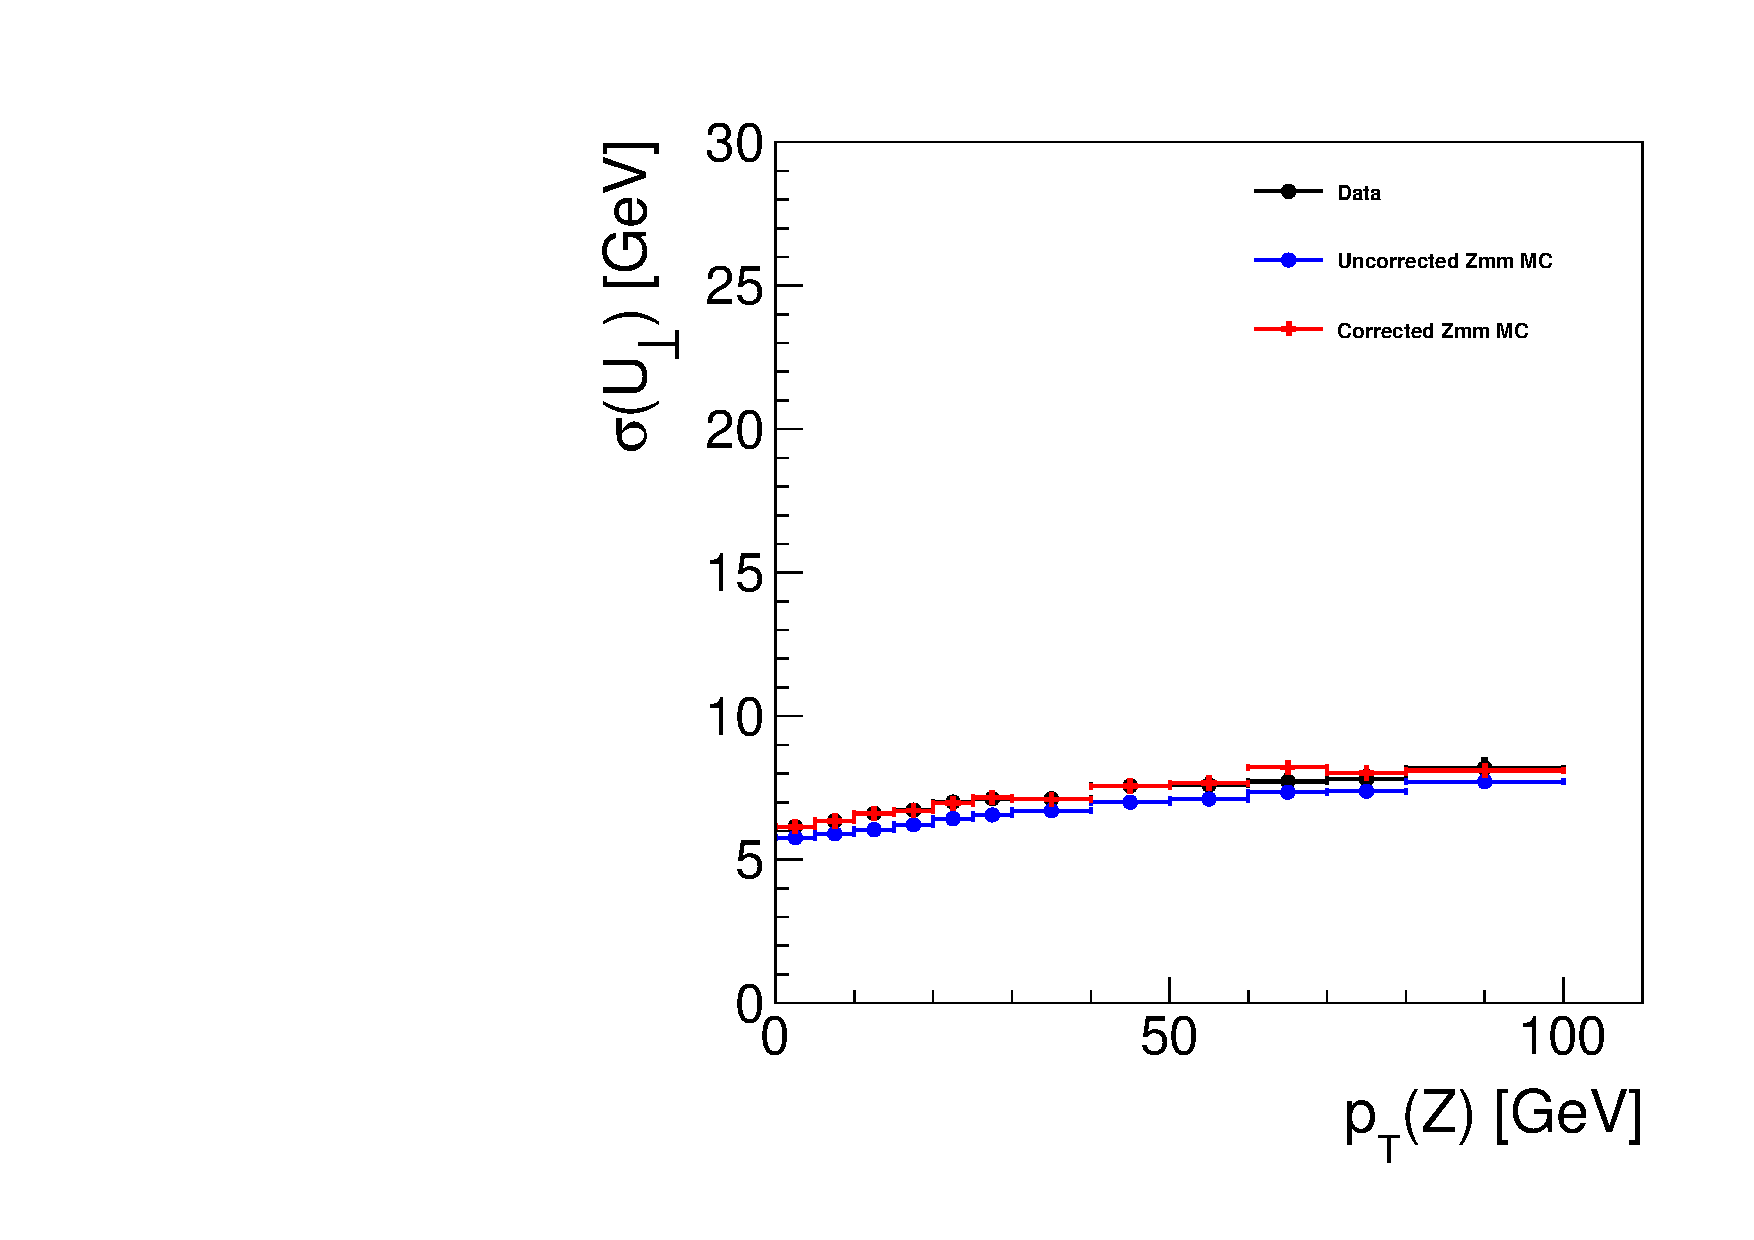
\includegraphics[width=\linewidth]{plots/Recoil/validation_5/resolution_prp.pdf}
\caption{Resolution of \uprp}
%   \caption{1a}
%   \label{fig:Eff:el:5TeV:GSFSel:pos
\end{subfigure}%
\\
\centering
\begin{subfigure}{.50\textwidth}
\centering
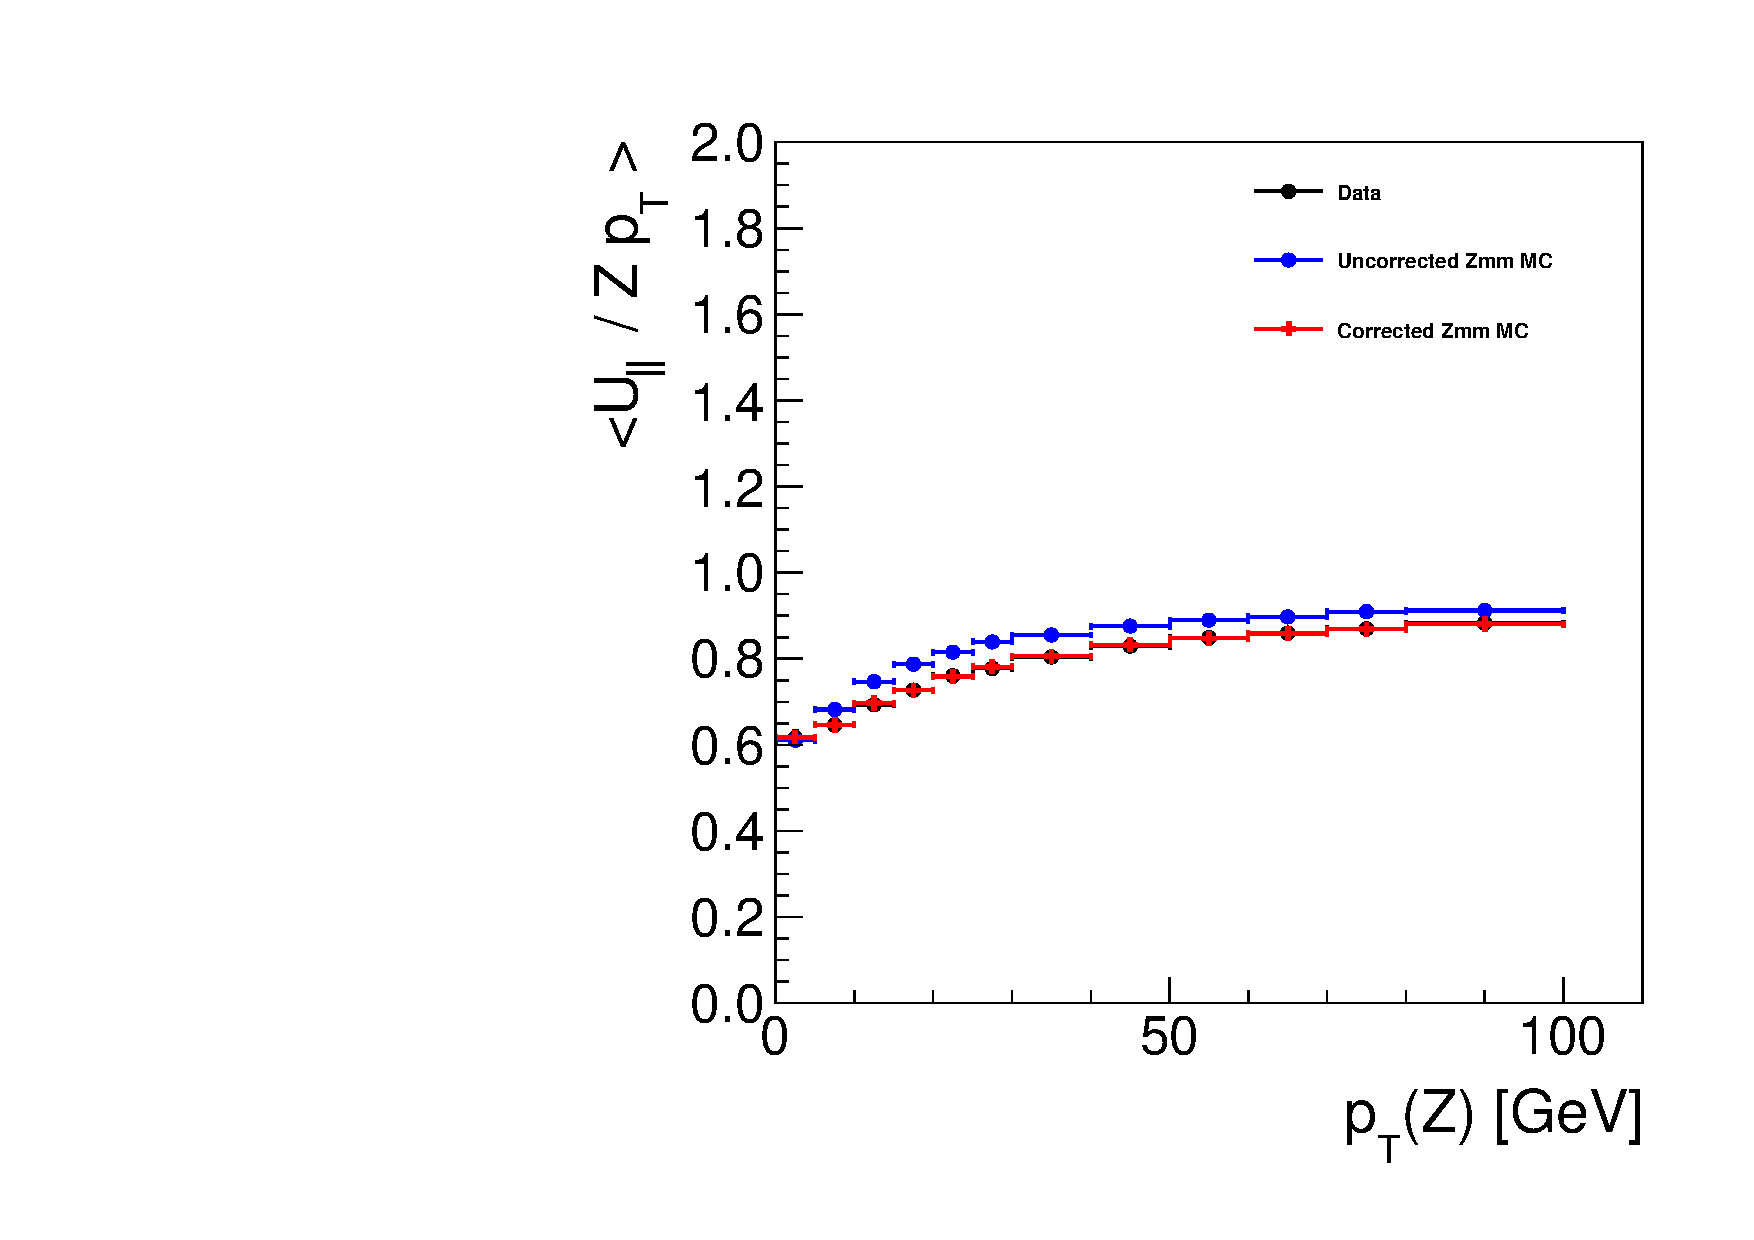
\includegraphics[width=\linewidth]{plots/Recoil/validation_5/response_par.pdf}
\caption{$p_T$-corrected response of \upar}
%   \caption{1a}
%   \label{fig:Eff:el:5TeV:GSFSel:pos
\end{subfigure}%
\caption{Closure of the recoil corrections derived from and applied to $Z\rightarrow\mu\mu$ samples for the 5 TeV dataset. The raw recoil distribution in Monte Carlo [blue] is corrected [red] towards the target spectrum of data [black].}
\label{fig:recoil:validation:5}
\end{figure}